\section{Gaussian Processes}
\subsection{The Bayes optimal classifier}
Theoretically optimal (= most probable) classification.
Combine predictions of all hypotheses, weighted by their posterior probabilities: (where \(y_i\) is  a label from the set \(Y\) of classes)
\[
P(Y = y_k|X_1,\dots,X_n) = \frac{P(Y = y_k)\prod_{i} P(X_i|Y = y_k)}{\sum_j P(Y = y_j) \prod_i P(X_i|Y = y_j)}
\]
Naive Bayes Classifier:
\[
Y \leftarrow\arg\max_{y_k} P(Y = y_k)\prod_i P(X_i|Y = y_k)
\]
\subsection{Gaussian Distribution (1D)}
Norma distribution with mean \(\mu\) and variance \(\sigma^2\):
\[
p(x) = \mathcal{N}(x|\mu,\sigma^2) = \frac{1}{(2\pi\sigma^2)^{1/2}}\exp\left\{-\frac{1}{2\sigma^2}(x-\mu)^2\right\}
\]
\[
\mathbb{E}\left[x\right] = \mathbb{E}_{x \sim p}\left[x\right] = \int x\cdot p(x)\,dx = \mu
\]
\[
    \mathbb{E}\left[x^2\right] = \mathbb{E}_{x \sim p}\left[x^2\right] = \int x^2\cdot p(x)\,dx = \mu^2 + \sigma^2
\]
\[
\textbf{VAR}\left[x\right] = \mathbb{E}\left[x^2\right]-\mathbb{E}\left[x\right]^2 = \sigma^2
\]
\subsubsection{Mulitvariante Gaussian Distribution}
Gaussian defined over a vector \(x\) of continuous variables in a \(D\)-dimensional space with mean vector \(\mu\) and covariance matrix \(\Sigma\), where \(|\Sigma|\) is the determinant of \(\Sigma\).
\[
    p(\mathbf{x}) = \mathcal{N}(\mathbf{x} | \mu, \Sigma) = \frac{1}{(2\pi)^{D/2} |\Sigma|^{1/2}} \exp\left\{-\frac{1}{2} (\mathbf{x} - \mu)^T \Sigma^{-1} (\mathbf{x} - \mu)\right\}
\]
The quadratic form in the argument of the exponential is called \textbf{Mahalanobis distance}:
\[
\Delta = (\mathbf{x} - \mu)^T \Sigma^{-1} (\mathbf{x} - \mu)
\]
\subsection{Gaussian Processes}
A Gaussian process \(\mathcal{GP}\) is a stochastic process, i.e. a collection of random variables that are drawn from a infinite dimensional multivariate Gaussian distribution.
A stochastic process is a collection of random variables, \(\left\{h(x):x\in \mathcal{X}\right\}\) indexed by elements from some set \(\mathcal{X}\), known as the index set.
\subsubsection{Definition of a Gaussian Process\(\mathcal{GP}\)}
A Gaussian process is a stochastic process such that any finite subcollection of random variables has a multivariate Gaussian distribution(mean function \(m(\cdot)\) and convariance function \(k(\cdot,\cdot)\))
\[
\begin{bmatrix}
h(x_1) \\
\vdots \\
h(x_m)
\end{bmatrix}
\sim \mathcal{N} \left(
\begin{bmatrix}
m(x_1) \\
\vdots \\
m(x_m)
\end{bmatrix},
\begin{bmatrix}
k(x_1, x_1) & \cdots & k(x_1, x_m) \\
\vdots & \ddots & \vdots \\
k(x_m, x_1) & \cdots & k(x_m, x_m)
\end{bmatrix}
\right)
\]
 
\subsubsection{Example}
One dimensional Gaussian process:
\[
p(f(x))\sim \mathcal{GP}\left\{m(x) = 0,k(x,x') = \exp\left(-\frac{1}{2}(x-x')^2\right)\right\}
\]
To get an indication of what this distribution over functions looks like, focus on a finite subset of function values \(\textbf{f} = (f(x_1),f(x_2),\dots,f(x_n))\) for which:
\[
    \textbf{f} \sim \mathcal{N}(0,\Sigma)
\]
\[
\Sigma_{ij} = k(x_i,x_j)
\]
Then plot the coordinates of \textbf{f} as a function of the rorresponfing \(x\) values
\begin{figure}[!h]
    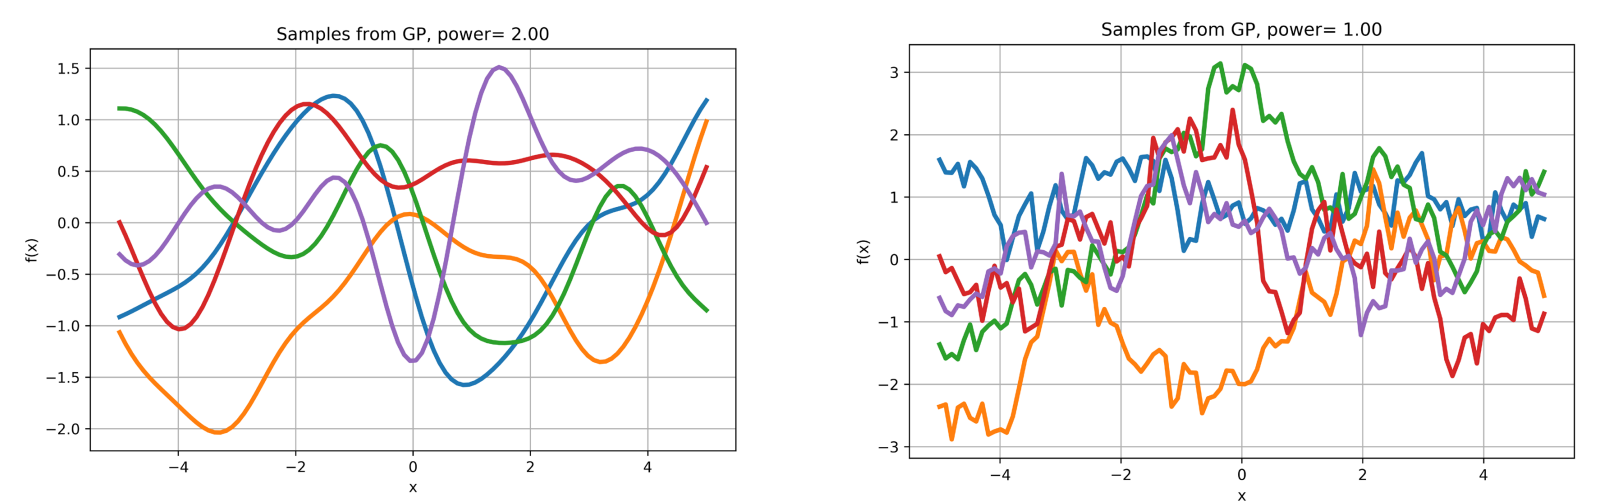
\includegraphics[width = \columnwidth]{figures/09/GPExample.png}
\end{figure}
\subsection{Covariance Function\(k(x,x') = \)Merver kernel}
Gaussian processes are kernel-based probability distribution in the sense that any valid kernel function can be used as a covariance function.
\(k(x,x')\) is a kernel, if there is a feature mapping \(\phi(x)\) into some (higher dimensional) space \(\mathcal{H}\), where it can be represented by a scalar (dot) product.

Some possible Kernels:
\begin{itemize}
    \item Radial Basis Function kernel (RBF)
    \[
    k(x,x') = \sigma_0^2\exp\left[-\frac{1}{2}(\frac{x-x'}{\lambda})^2\right]
    \]
    \item Rational-Quadratic kernel
    \[
    k(x,x') = \left(1 + \frac{(x-x')^2}{2\alpha\lambda^2}\right)^{-\alpha}
    \]
    \item Exp-Sine-Squared kernel
    \[
    k(x,x') = \exp\left[-\frac{2 \cdot \sin^2(\pi/p \cdot |x-x'|)}{\lambda^2}\right]
    \]
    \item Dot-Product kernel
    \[
    k(x,x') = \sigma^2_0 + x\cdot x'
    \]
\end{itemize}

\subsection{Important information}
\begin{itemize}
    \item MAP assignment: The Most porbable A Posteriori (MAP) setting is thta which maximises the posteriori. It is the most probable set of parameters \(\theta\) given the Data \(\mathcal{D}\) and model class \(\mathcal{M}\)
    \[
    \hat{\theta}_{\text{MAP}} = \arg\max_\theta\{p(\theta|\mathcal{D},\mathcal{M})\} = \arg\max_\theta \{p(\theta,\mathcal{D}|\mathcal{M})\}
    \]
    \item Max. Likelihood assignment: when \(p(\theta|M) = \)const. It is the estimate for \(\theta\) that maximises the probability of observing the data \(\mathcal{D}\) given the model \(M\).
    \[
    \hat{\theta}_{\text{ML}} = \arg\max_\theta\{p(\mathcal{D}|\theta,\mathcal{M})\}
    \]
\end{itemize}
Matrix inverse:
\[
A = 
\begin{bmatrix}
a & b \\
c & d
\end{bmatrix}
\qquad
A^{-1} = \frac{1}{\text{det}(A)}
\begin{bmatrix}
d & -b \\
-c & a
\end{bmatrix}
\]
